
\chapter{مقدمه}
\section{معرفی برنامه مورد آزمون و هدف پروژه}

برنامه مورد ازمون یک پروژه به زبان جاوا می‌باشد که وظیفه آن ترجمه برنامه ورودی به یک کد میانی ۳ آدرسه است. این کامپایلر تک گذره برای زبان MiniJava طراحی شده است. که این زبان قابلیت‌های کمتری نسبت به زبان جاوا دارد و زبان کوچکتری نسبت به آن محسوب می‌شود. این پروژه شامل ۵ قسمت اصلی می‌باشد: ۱. تحلیل گر لغوی ۲. تحلیل گر نحوی ۳. تحلیل گر معنایی ۴. مولد کد میانی  ۵. خطا پرداز 

این پروژه یک متن حاوی برنامه ای به زبان MiniJava را به عنوان ورودی قبول می‌کند و آن را ترجمه می‌کند و کد‌های میانی ۳ آدرسه به شرح تصویر \ref{fig:1} را تولید می‌کند.

\begin{figure}[ht]
\centering
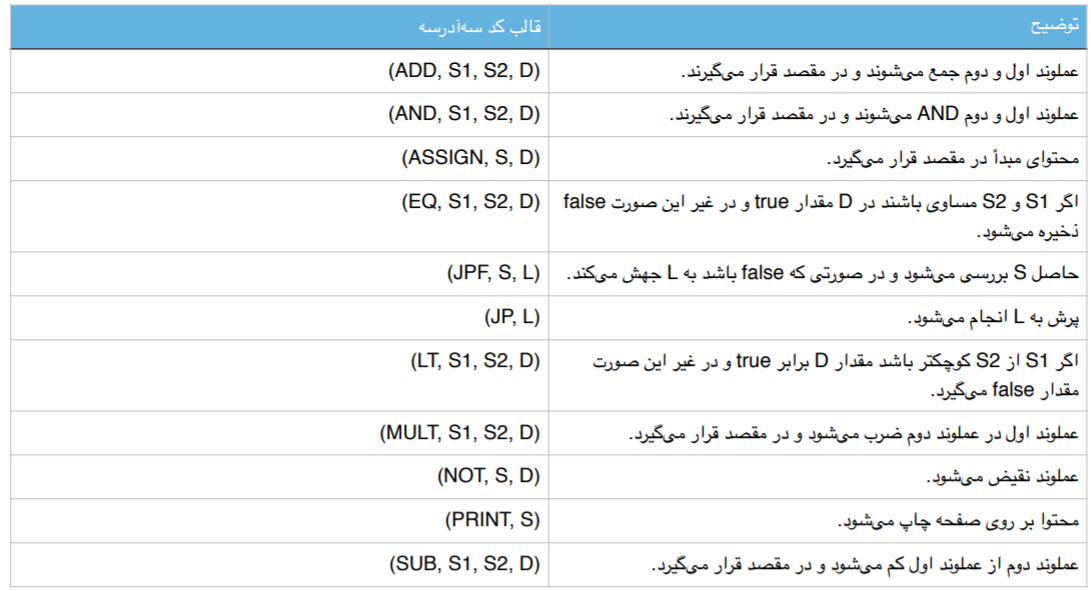
\includegraphics[scale=0.8]{3add.PNG}
\caption{کد‌های ۳ آدرسه}
\label{fig:1}
\end{figure}



حال به عنوان کسانی که آزمون نرم‌افزار می‌دانند از ما خواسته شده که این پروژه را آزمون کنیم با این هدف که اگر خطایی در این برنامه وجود دارد ان خطا را به تیم برنامه نویس پروژه اعلام کنیم و همچنین توضیح دهیم که چرا این آزمون خوب است و چقدر خوب است و چگونه طراحی شده است.
از انجا که هدف این آزمون رفع‌یابی خطاهای پروژه توسط خود تیم آزمون نیست تنها موارد آزمون مناسب باید طراحی شود.
همچنین گفته شده است که قرار نیست که برای تک تک توابع در این پروژه آزمون نوشته شود و یک راه حل مناسب و منطقی ارائه شود. 

\section{فرض‌ها و محدودیت‌های درنظر گرفته شده}\label{sec:limit}
کد برنامه کامپایلر MiniJava خود بر اساس گرامر MninJava نوشته شده است که این گرامر به عنوان توصیف صحیح ما از کاری است که قرار است این برنامه انجام دهد، البته دقت شود که همه برنامه‌هایی که با این گرامر ساخته می‌شود، برنامه مورد قبول ما نیست و باید شروط دیگری که در ضمن کد نیز گذاشته شده است نیز رعایت شود. 
برای مثال این که این گرامر تک گذره است و اشاره‌ای رو به جلو رخ نباید بدهد یا identifier نباید جزو کلمات کلیدی ای مانند int یا class باشد یا اگر در ادامه identifier ای استفاده شد باید قبل از آن تعریف شده باشد یا به شیوه صحیح call شود یا دستور چاپ تنها محتوی عدد صحیح را چاپ کند.
به همین منظور ازمون‌های مورد نیاز ورودی به برنامه ابتدا از طریق گرامر MiniJava ساخته می‌شوند و در حین ساخت به این موارد نیز توجه می‌شود (که البته تمامی specification برنامه دست ما نیست و این موارد جزو فرضیات اضافه برای شروع آزمون است).

همچنین فرض دیگر نیز آن است که  برای اعداد ‌int رقم‌های ۰ تا ۹ و برای literal ها ترکیب حروف کوچک و بزرگ انگلیسی در نظر گرفته شده است.


\section{روش آزمون انتخابی و دلایل انتخاب آن}\label{sec: method}

متدهای مختلفی برای تست این برنامه وجود دارد؛ برای مثال برای قسمتی از برنامه که دارای قواعد شروط اما و اگر زیاد است می‌توان از آزمون منطق یا برای مثال در قسمت‌هایی که شامل حلقه است و برنامه پیچیدگی‌های الگوریتمی دارد از روش‌های مبتنی بر گراف و اگر برای مثال اگر تابع مورد بررسی حالت واسط دارد از روش‌های واسط  می‌توان استفاده کرد.  
در ادامه خواهیم دید که چه روشی انتخاب شده و دلیل انتخاب این روش چه بوده است.

اما همانجور که قبلا گفته شد از آنجا که بهترین توصیفی که از برنامه داریم توسط گرامر به ما داده شده است، بهترین آزمون آن است که بر اساس این گرامر و فرضیات اضافه مساله ورودی معتبر را تولید کنیم و سپس آن را به به عنوان مورد آزمون به برنامه بدهیم با توجه به توصیف برنامه از کد‌های میانی نیز می‌توانیم خروجی مورد انتظار معتبر را تولید کنیم. 

به طور کلی از دلایل انتخاب می‌توان به موارد زیر اشاره کرد:

\begin{itemize}
\item
از آنجا که گرامر به عنوان توصیف صحیح از برنامه حضور دارد بهترین راه برای تست استفاده مستقیم از خود گرامر برای تولید ورودی‌های معتبر است، از انجا که خروجی مورد معتبر نیز با توجه به شکل \ref{fig:1} قابل دستیابی است این روش را ممکن می‌کند. 

\item
کد بخش های مختلفی دارد و پیچیدگی بسیاری در برخی از بخش‌ها دارد، همچنین به ازای هر تابع مجزا توصیفی از کار تابع، ورودی ها و خروجی‌های مورد انتظار وجود ندارد و این موضوع موجب می‌شود که تست تابع به تابع امکان پذیر نباشد. در صورتی که روش پیشنهاد شده نیاز ندارد تا به صورت مجزا توصیف تابع‌ها را بداند و با هر مقدار پیچیدگی در بالاترین سطح ممکن می‌تواند کد را بیازماید و اگر رفتار آن متفاوت با خروجی مورد انتظار بود آن را گزارش دهد. 

\end{itemize}

\section{معیارهای پوشش انتخابی}\label{sec: method2}
از انجا که در این آزمون از گرامر استفاده می‌کنیم از معیار پوشش production استفاده می‌کنیم. در این پوشش باید هر یک از قوانین گرامر حداقل یکبار trigger شوند، حداکثر تعداد موارد ازمون طراحی شده با این روش برابر تعداد قوانین هر گرامر است. 


\section{چگونگی استفاده از روش‌های انتخابی}\label{sec: method3}

ابتدا گرامر به فرم استانداردی که که در آن غیرترمینال‌ها با "" مشخص شده است در می‌آوریم. همچنین به هر یک از قوانین شمار‌ه‌ای داده شده است تا شمارش و رفرنس‌دهی راحت تر باشد. برای معادل کردن گرامر دو قانون ۵۳ و ۵۴ را به فرمی که در شکل \ref{fig:2} (یا فایل grammar.bnf به پیوست) مشاهده می کنید بازنویسی شده است و در نهایت به ۱۲۰ قانون مجزا دست پیدا شده است. 

\begin{figure}[ht]
\centering
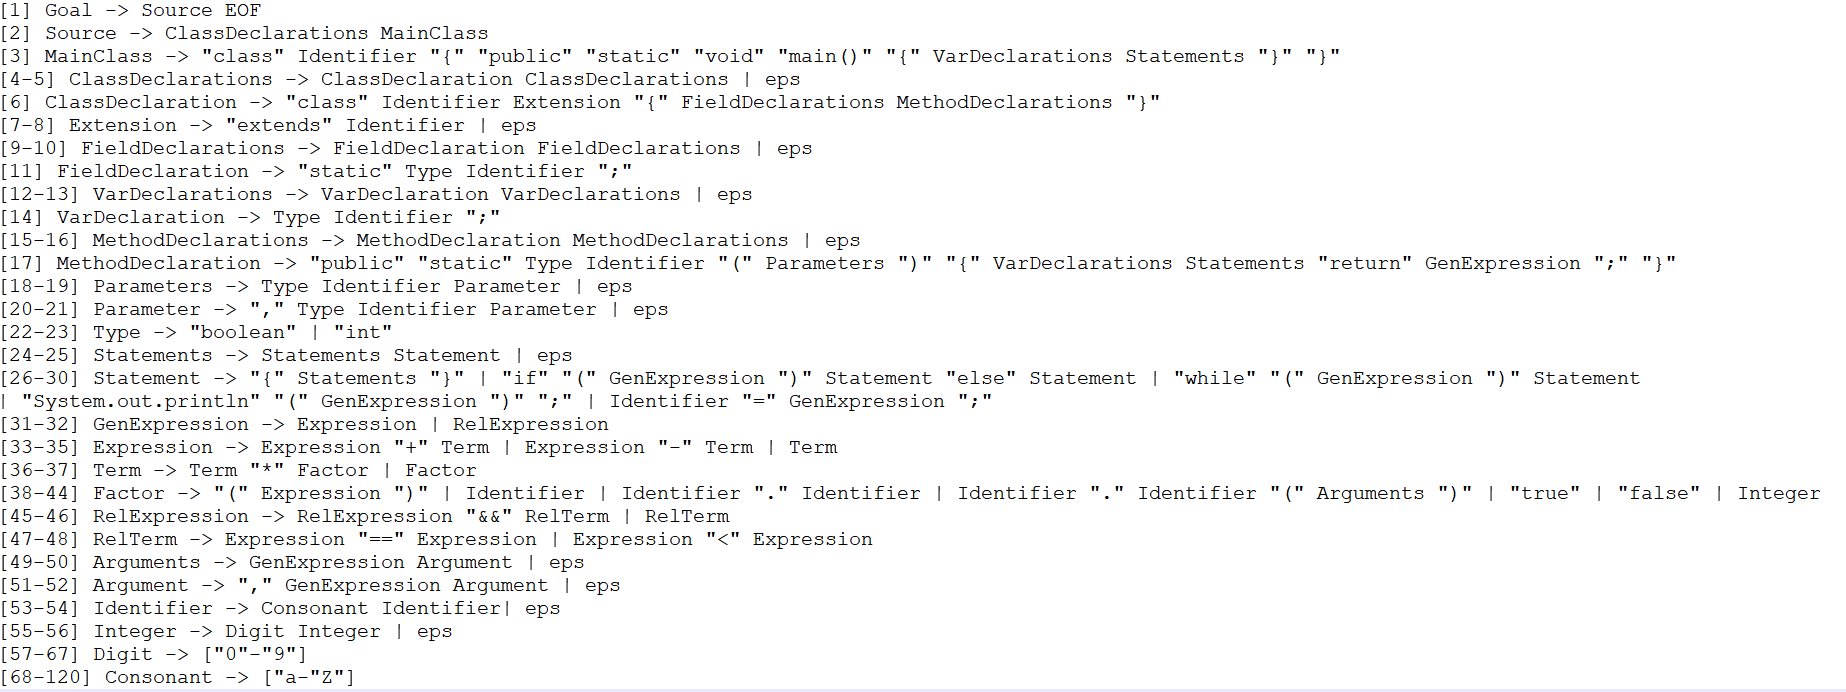
\includegraphics[scale=0.32]{grammar.png}
\caption{گرامر bnf}
\label{fig:2}
\end{figure}

در ادامه با استفاده از این گرامر سعی شده است که یک یا چند کد تولید شود که تا حد ممکن از تمامی قوانین در مجموع کدهای تولیدی استفاده شده باشد. پکیج‌هایی نظیر nltk وجود دارند که می‌توان گرامر را با همین فرمت دریافت کنند و از قوانین آن رشته‌های مختلف با عمق متفاوت بسازند، اما از آنجا که این پکیج‌ها عموما محدودیت‌هایی دارند که ملزم به cfg بودن گرامر و نداشتن recursion می‌کند به همین منظور ترجیح داده شد با توجه به این نوع محدودیت‌های بیان شده در بخش \ref{sec:limit} مورد آزمون به صورت دستی نوشته شود، در نهایت یک مورد آزمون نوشته شد که از تمامی قوانین در آن استفاده شده است، در بسط دادن تا جای ممکن از اشتقاق سمت چپ استفاده شده است. بدلیل طولانی بودن بسط دادن تنها چند مرحله اول و خروجی نهایی نشان داده شده است.


\begin{figure}[ht]
\centering
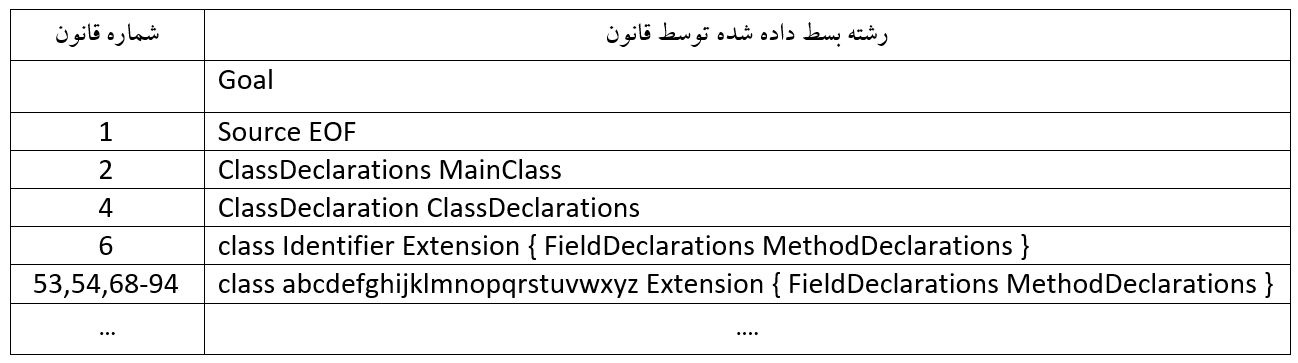
\includegraphics[scale=0.6]{derivation.PNG}
\caption{بسط گرامر توسط قوانین}
\label{fig:3}
\end{figure}

\begin{figure}[ht]
\centering
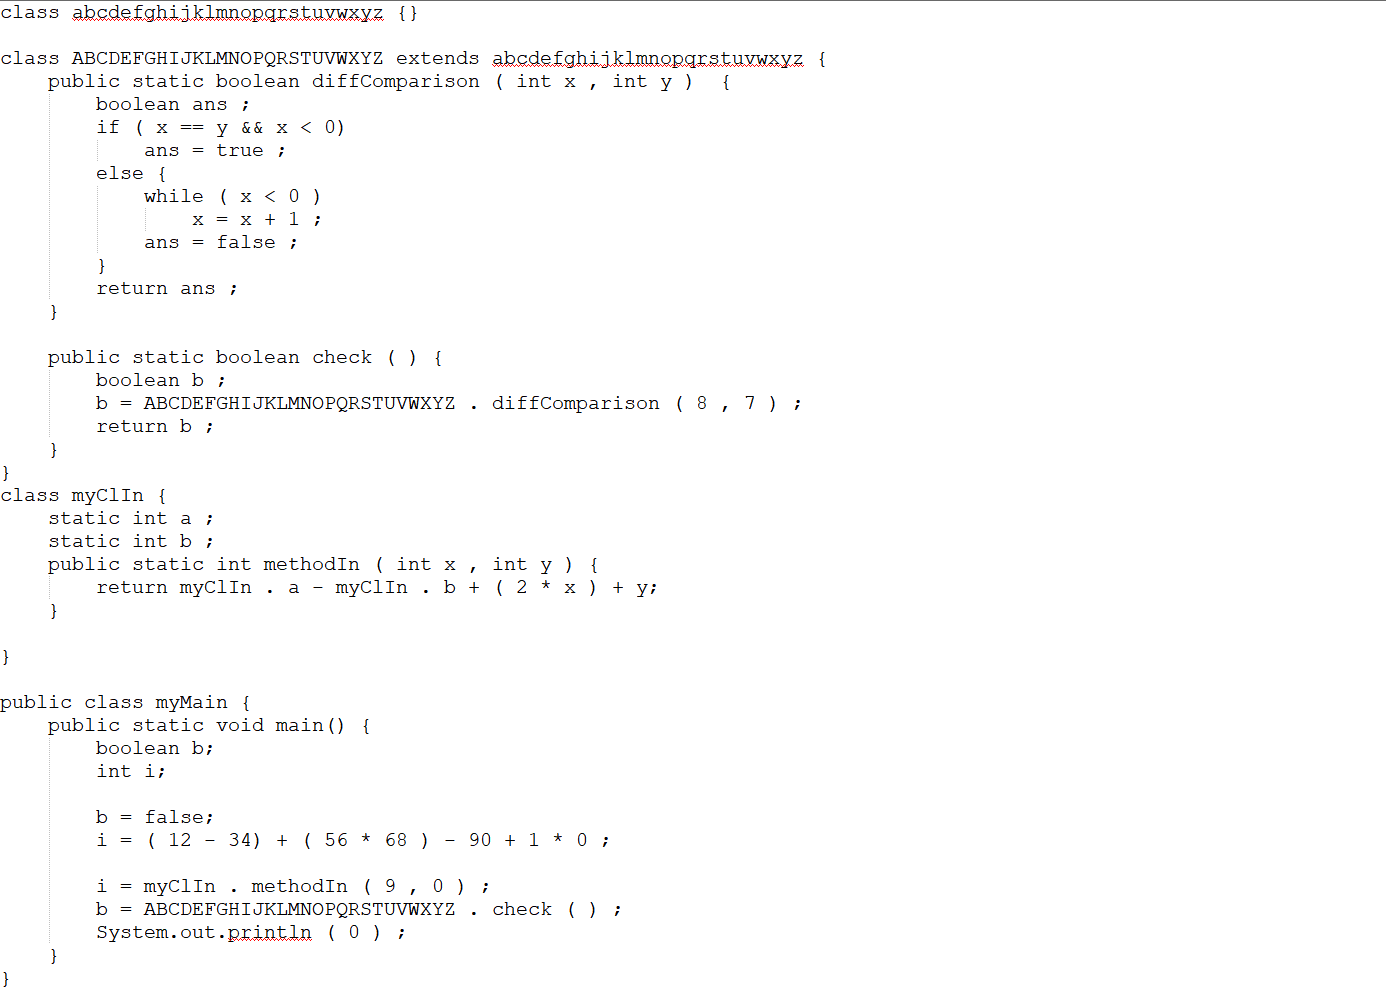
\includegraphics[scale=0.6]{output_test.PNG}
\caption{خروجی بسط گرامر با تریگر کردن تمام قانون ها حداقل یکبار}
\label{fig:4}
\end{figure}

\section{ابزارهای مورد استفاده جهت تست}
\begin{itemize}
\item Junit: برای اجرای تست‌ها 
\item PIT : برای ایجاد موتاسیون و اندازه‌گیری پوشش
\end{itemize}


\section{مراحل مختلف آزمون}
همانگونه که در بخش \ref{sec: method} گفتیم از روش گرامر برای تولید آزمون استفاده خواهیم کرد و همانطور که در بخش \ref{sec: method2} گفتیم پوشش مد نظر پوشش production خواهد بود که از جمله‌ پوشش‌های قوی‌ برای گرامر‌هاست و همانگونه که در بخش \ref{sec: method3} گفتیم مورد آزمون همانند شکل \ref{fig:3} بسط می‌یابد و از هر قانون حداقل یکبار استفاده می‌شود و خروجی نهایی آن بدست می‌اید که در شکل \ref{fig:4} نمایش داده شده است.  
نهایتا آزمون با استفاده از ابزار Junit اجرا می‌شود و diff خروجی و خروجی مورد انتظار گرفته و بررسی می‌شود. همچنین از ابزار PIT برای ایجاد موتاسیون استفاده می‌شود تا مشخص شود که چه قسمت‌هایی از کد پوشش داده شده است و تست طراحی شده چقدر مناسب است.

\subsection{نیازمندی‌های آزمون}
با توجه به انتخاب پوشش production نیازمندی‌های آزمون P1 تا P120 می‌باشد که متناظر هر یک از قوانین داخل گرامر است.

\subsection{مورد آزمون}
مورد آزمون رشته تولید شده توسط گرامر و پوشش production است که در شکل \ref{fig:4} نمایش داده شده است.

در طراحی مورد آزمون باید خروجی مورد انتظار نیز نمایش داده شود که خروجی مورد انتظار برای این رشته در شکل \ref{fig:5} نمایش داده شده است.

\begin{figure}[ht]
\centering
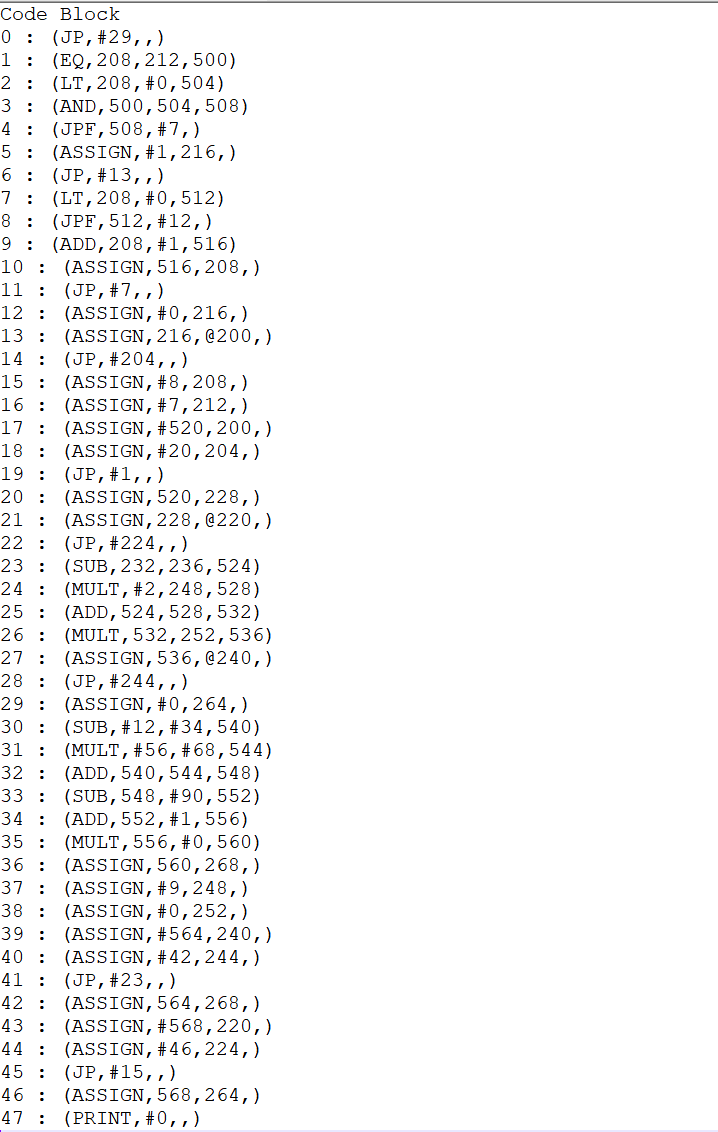
\includegraphics[scale=0.6]{output.PNG}
\caption{خروجی مورد انتظار مورد آزمون طراحی شده}
\label{fig:5}
\end{figure}



\subsection{انجام آزمون}
\subsubsection{:Junit}

با استفاده از junit و assertion مساوی خروجی کد رو ابتدا در فایل print.txt ریخته و سپس با آنچه که به عنوان خروجی موردنظر طراحی شده است مقایسه می‌کند. همانگونه که در شکل \ref{fig:6} مشاهده می‌شود، تست انجام شده و جواب خروجی و جواب مدنظر مقایسه شده و خطا raise شده است، در کنسول خطا تصویر \ref{fig:6} کاملا مشخص است.
\begin{figure}[ht]
\centering
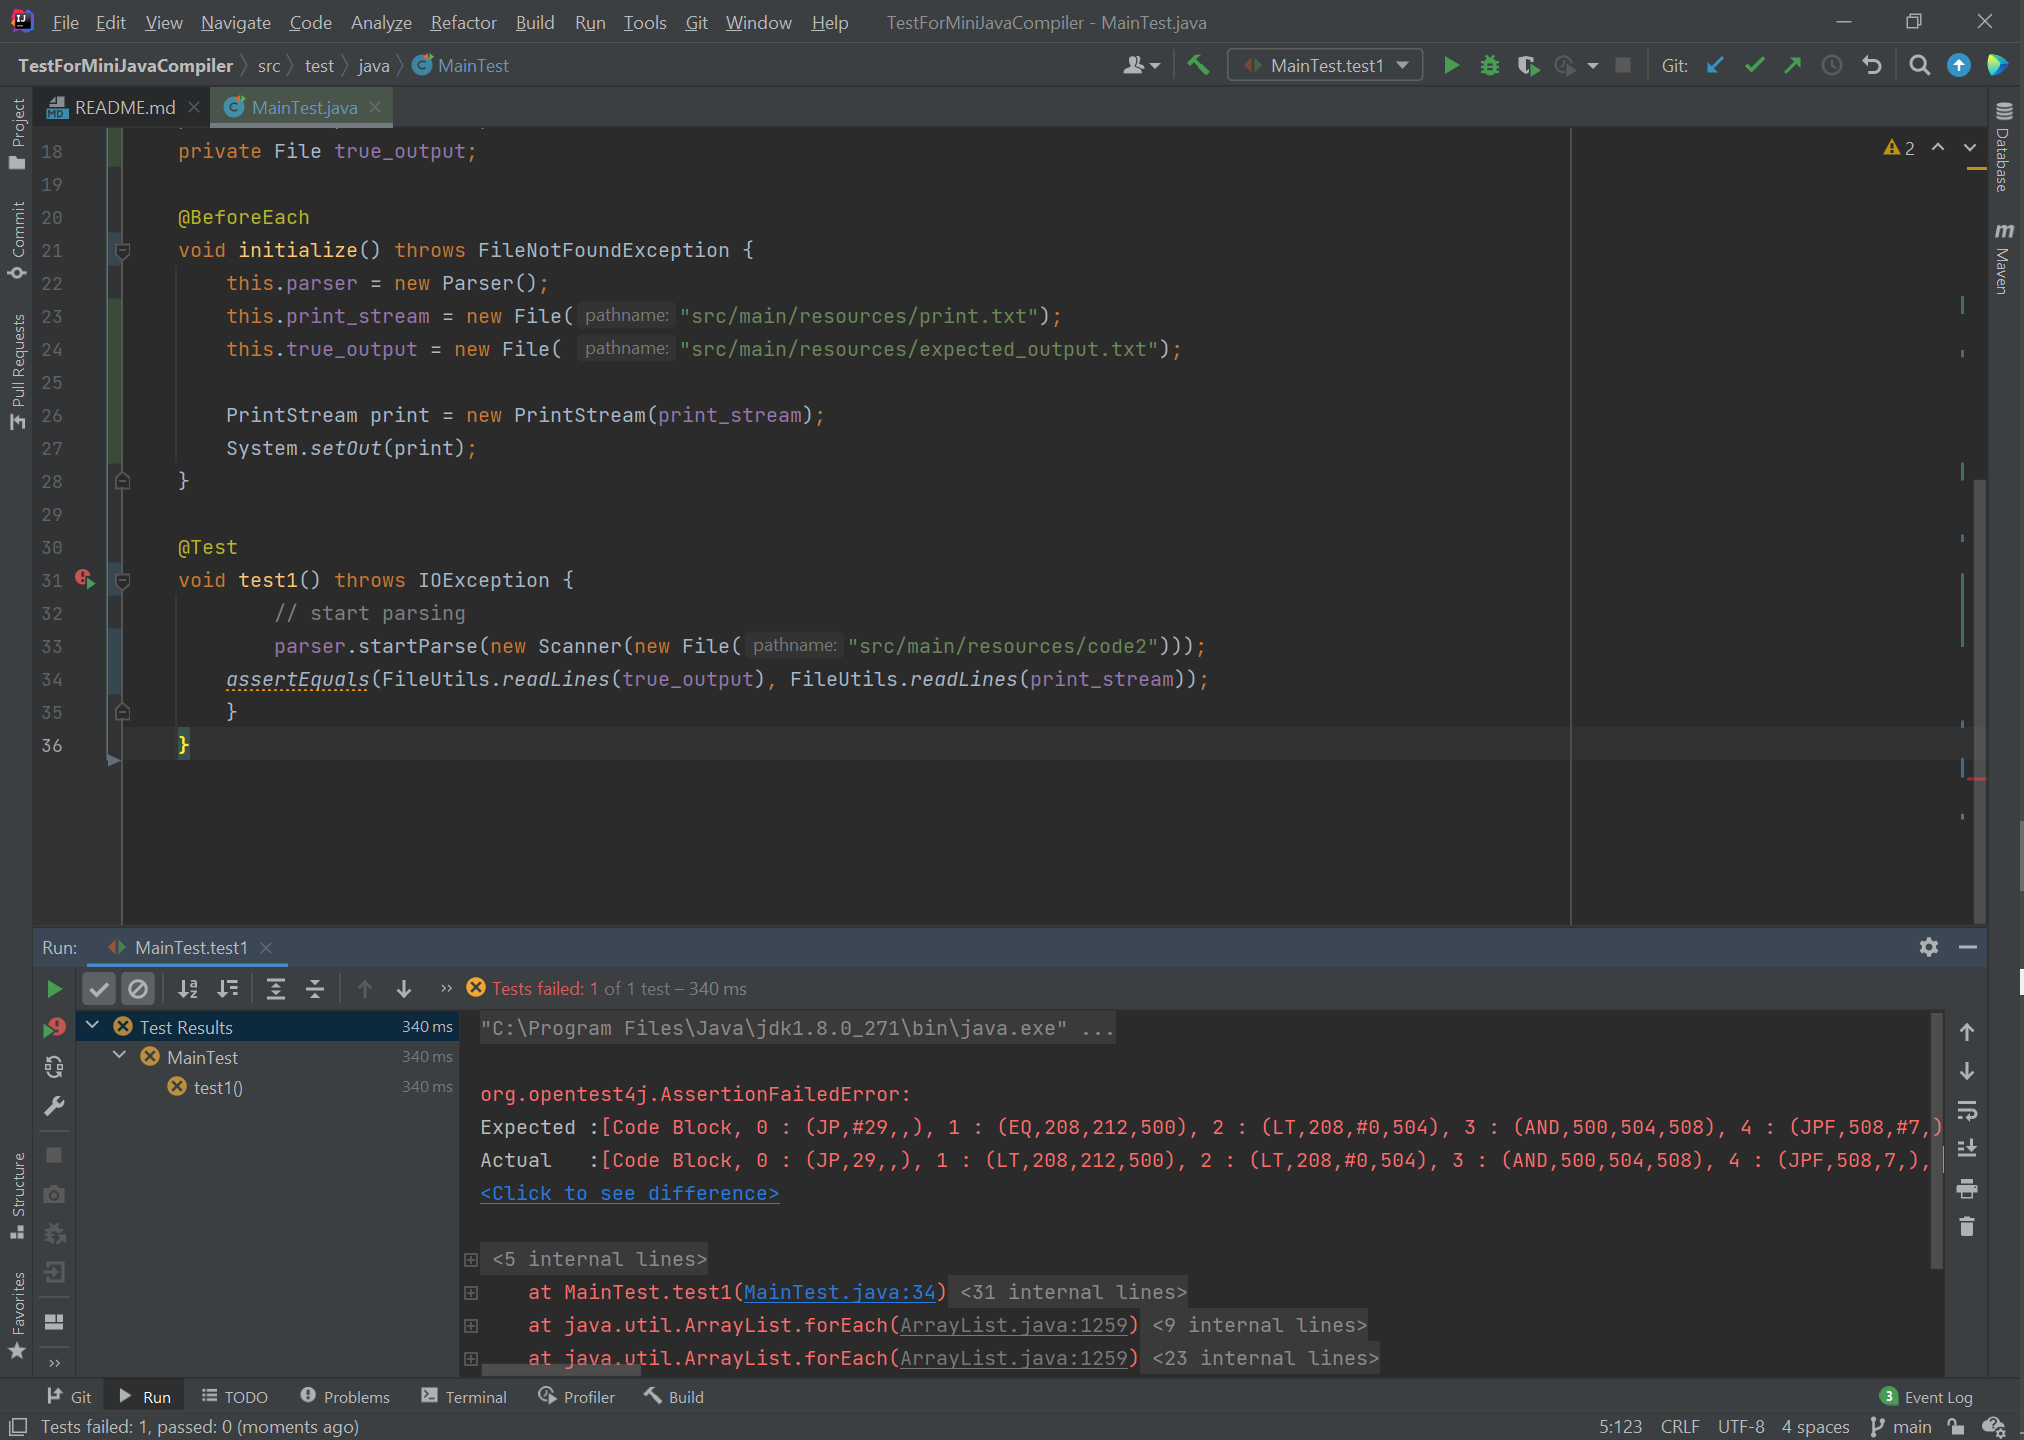
\includegraphics[scale=0.35]{test.PNG}
\caption{انجام آزمون}
\label{fig:6}
\end{figure}


اگر دو فایل را با یکدیگر مقایسه کنیم متوجه خطاها به صورت خط به خط می‌شویم، مقایسه این دو را در شکل \ref{fig:7} مشاهده می‌کنید.

\begin{figure}[ht]
\centering
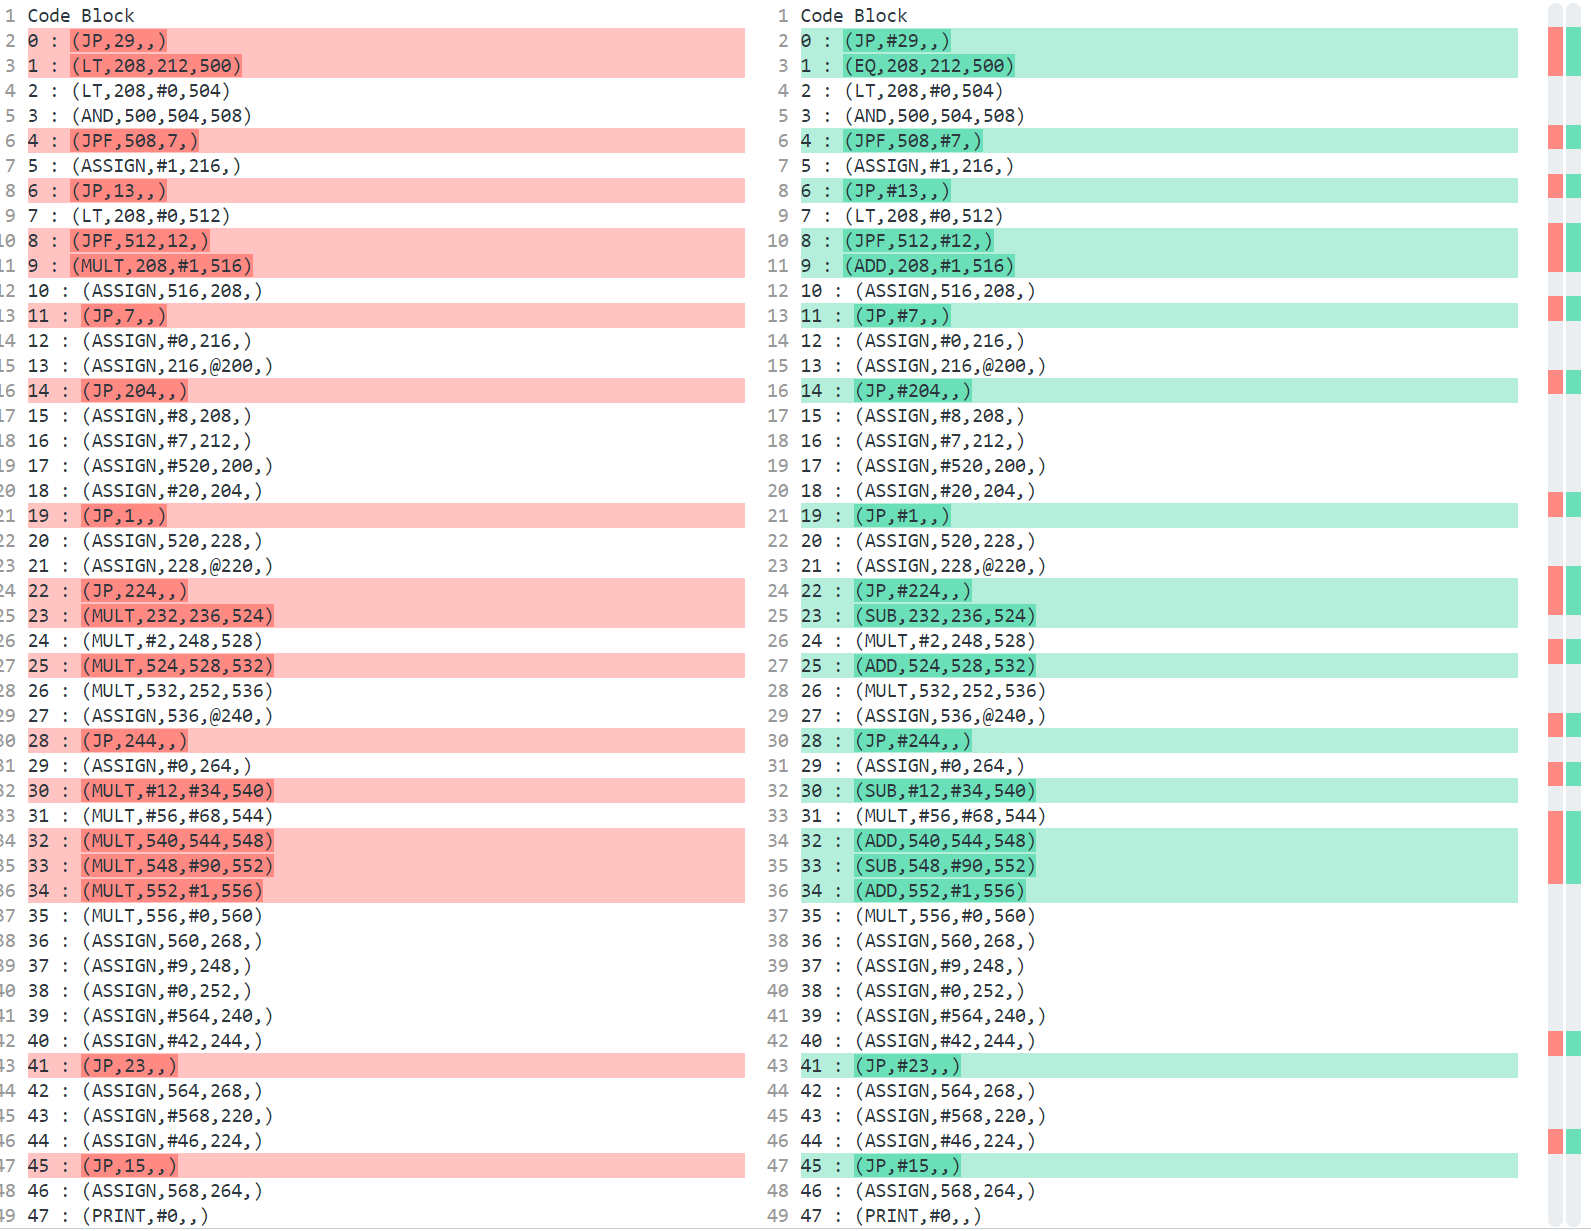
\includegraphics[scale=0.5]{diff.PNG}
\caption{مقایسه فایل خروجی و فایل مورد انتظار}
\label{fig:7}
\end{figure}

\subsubsection{:PIT}

بدون رفع کردن خطاهای موجود در برنامه از ابزار PIT برای آزمون موتاسیون استفاده می‌کنیم. این ابزار نیاز دارد که یک سری mutator را به عنوان کانفیگ دریافت کند، که تعدادی پیش‌فرض آن را انتخاب کردیم که فعال‌های آن در این پروژه در شکل \ref{fig:9} مشاهده می‌کنید، همچنین کلاس‌های هدف رو نیز تعیین کرد که در شکل \ref{fig:8} کلاس‌های هدف تعیین شده را مشاهده می‌کنید.
\begin{figure}[ht]
\centering
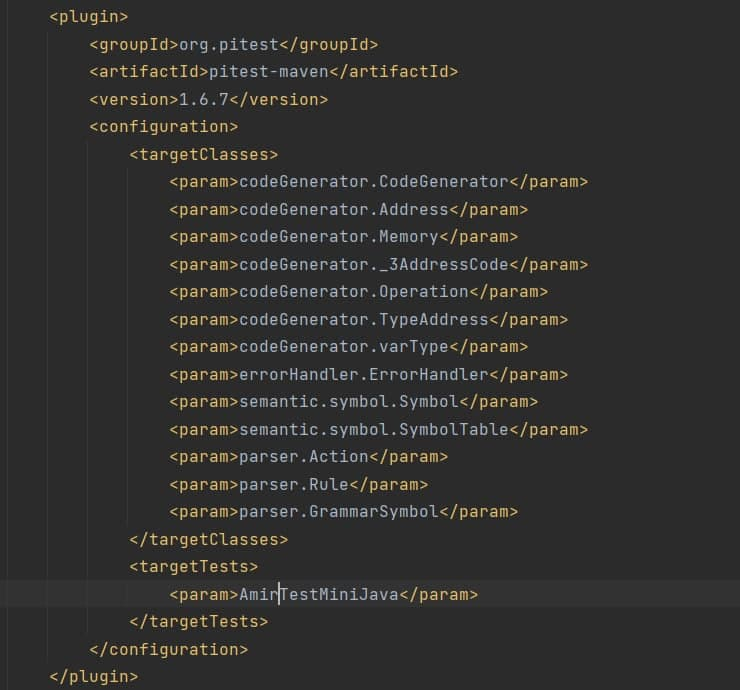
\includegraphics[scale=0.5]{PIT1.jpg}
\caption{کلاس‌های تعیین شده در PIT}
\label{fig:8}
\end{figure}

\begin{figure}[ht]
\centering
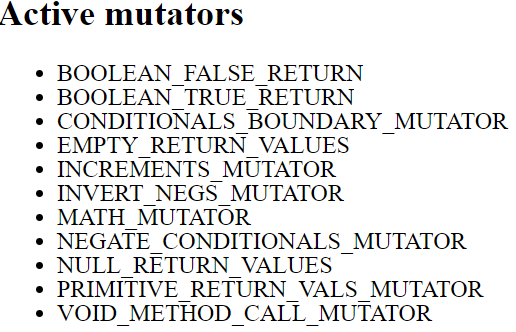
\includegraphics[scale=0.8]{PIT2.png}
\caption{mutator های فعال}
\label{fig:9}
\end{figure}


توسط این ابزار می‌توان ریپورت جامعی را با پسوند html تولید کرد که نشان می‌دهد چه تعداد موتاسیون تولید شده و چه تعداد از آن‌ها توسط تست پیشنهاد شده پوشش داده شده است. 
در شکل زیر نمای کلی این گزارش را مشاهده می‌کنید. 

\begin{figure}[ht]
\centering
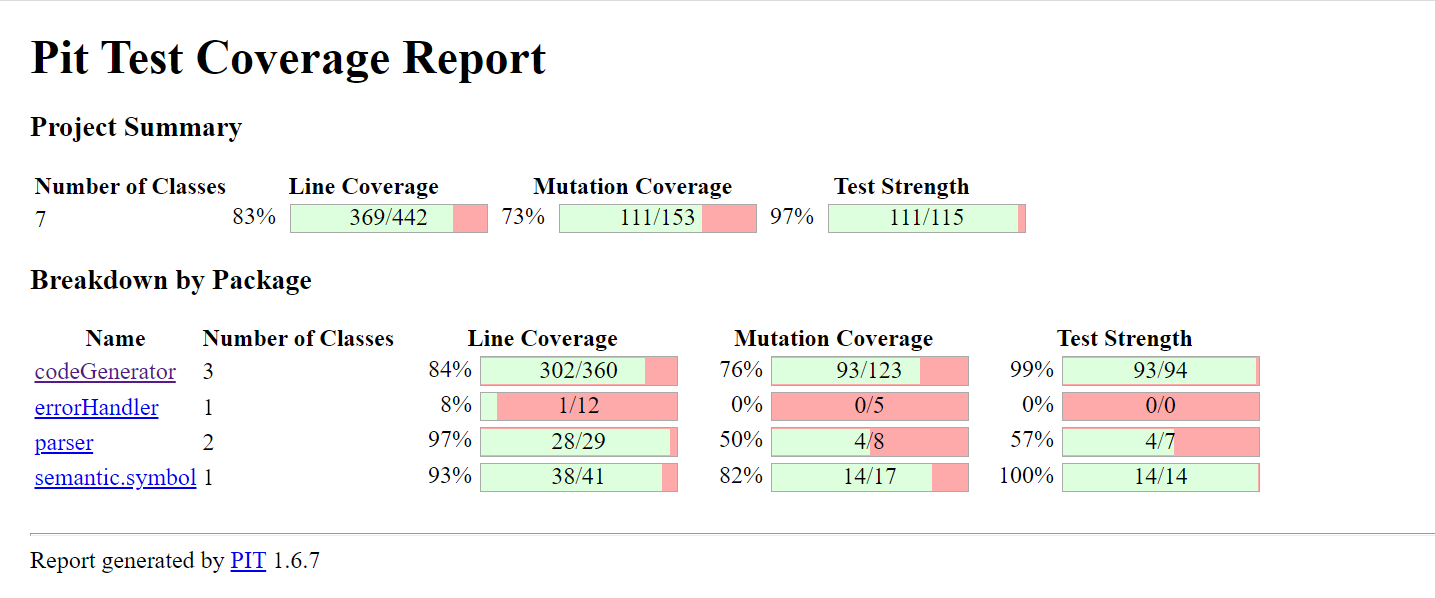
\includegraphics[scale=0.5]{PIT3.png}
\caption{آزمون موتاسیون}
\label{fig:9}
\end{figure}


در برخی از موارد پوشش کامل نیست و به این منظور به داخل ریپورت‌ها مراجعه می‌کنیم و خطوط قرمز رنگ را بررسی و وضعیت ان‌ها نسبت به خطوط سبز را می‌سنجیم.
ماژول errorHandler که طبیعی است چرا کمترین پوشش را دارد، چون که در ازای اجرای این تست ما به خطا نمی‌خوریم و بیشتر خطوط این ماژول برای مدیریت خطاهاست. همچنین وقتی به داخل ماژول semantic.symbol می‌رویم تنها خطوط قرمز مربوط به مدیریت خطاهای مربوط به آن مانند خطاهای مروبط به دوباره تعریف کردن نام یک کلاس متد یا متغیر است و بقیه خطوط پوشش داده شده است.
در parser هم که فقط فایل Action.java کامل پوشش داده نشده که یه switch بوده که مشخصا خطا از آنجا نیز نیست. تنها کلاس باقی مانده CodeGenerator است که وقتی داخل آن می رویم به وضوح دیده می‌شود که در زیر فایل codegenerator.java  یک سری از توابع که مربوط به کد‌های میانی ADD ، SUB و EQ است که هیچ وقت صدا زده نشده‌اند حال آن که در مورد ازمون این موارد وجود داشتند که مشخصا نشان می‌دهد این کلاس به درستی کار نمی‌کند، جزییات را در شکل \ref{fig:10} مشاهده می‌کنید.

\begin{figure}[htb]
\centering
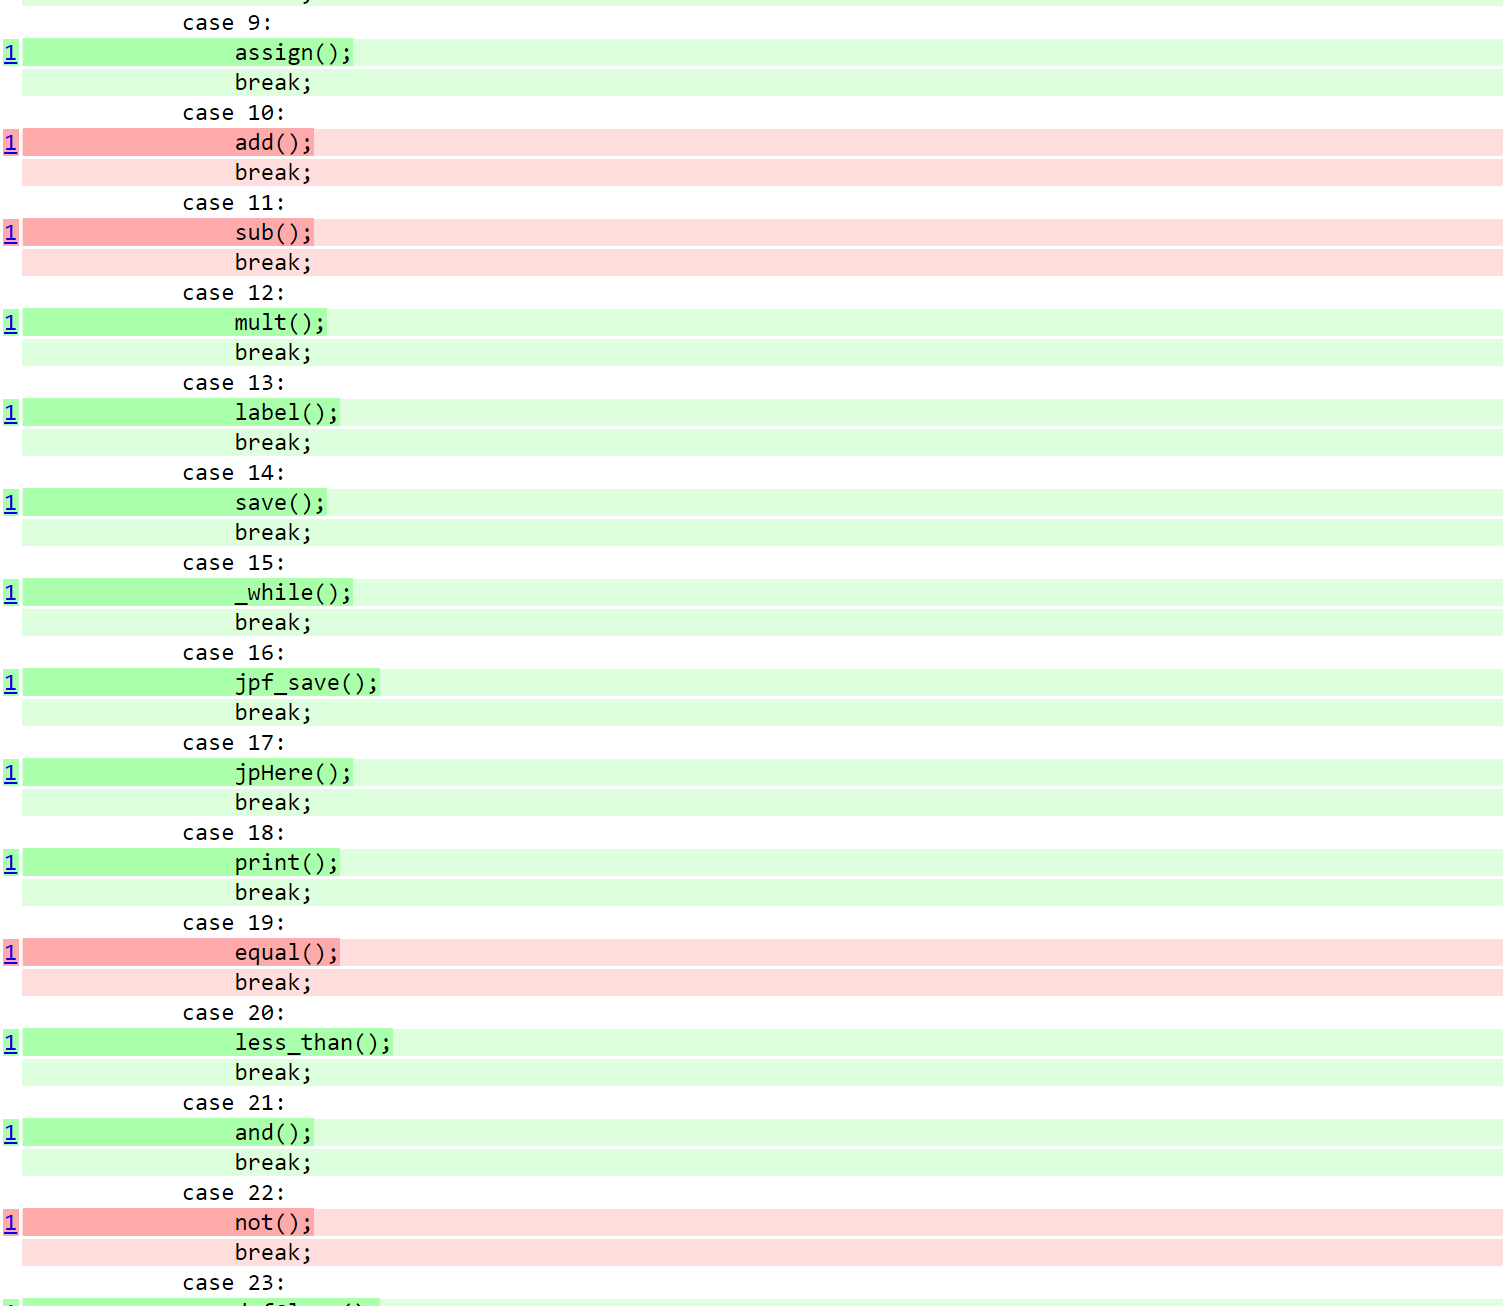
\includegraphics[scale=0.4]{PIT4.png}
\caption{آزمون موتاسیون فایل codegenerator.java}
\label{fig:10}
\end{figure}


\section{نتیجه‌گیری}

همانگونه که گفته شد مقایسه دو خروجی مورد آزمون و خروجی مورد انتظار در شکل \ref{fig:7} انجام شده است. 
از مقایسه چندین تفاوت بین خطوط ان‌ها متوجه می‌شویم که خروجی کامپایلر در این خطوط با یک دیگر فرق دارد:
\begin{itemize}
\item 
به جای EQ خروجی برابر LT می‌گذارد.
\item
به جای ADD و SUB خروجی برابر MULT می‌گذارد.
\item
در پرش‌ها علامت شارپ را فراموش می‌کند.
\end{itemize}

همچنین با استفاده از آزمون موتاسیون دیدیم که توابع متناظر همین خطاها در فایل codegenerator.java اصلا اجرا نمی‌شوند و پوشش داده نمی‌شوند. 

برای انجام کارهای بیشتر بهتر بود که خطاها درگام اول که شناخته می‌شدند برطرف می‌شدند و سپس آزمون موتاسیون اجرا می‌گردید و باز بررسی می‌گشت و دوباره به طراحی موارد آزمون می‌پرداختیم تا mutant بیشتری kill شود و با این طراحی مجددا خطاها را میافتیم و باز رفع می‌کردیم . دوباره آزمون موتاسیون را با تعداد بیشتری mutant اجرا می‌کردیم و این روند را به صورت چرخه تکرار می‌کردیم تا تعداد mutant هایی که kill می‌شوند افزایش یابد و اگر نسبت آن دیگر ثابت ماند پروسه رو متوقف می کردیم. با توجه به انتخاب این روش و عدم موجود بودن هر یک از توصیف تابع‌ها تصحیح خطاها سخت می‌انجامید. لذا به پیدا کردن این خطاها تا همین جا با استفاده از گرامر و پوشش production و انجام یک تست جامع با استفاده از Junit و PIT  و گزارش آن بسنده کردیم.
